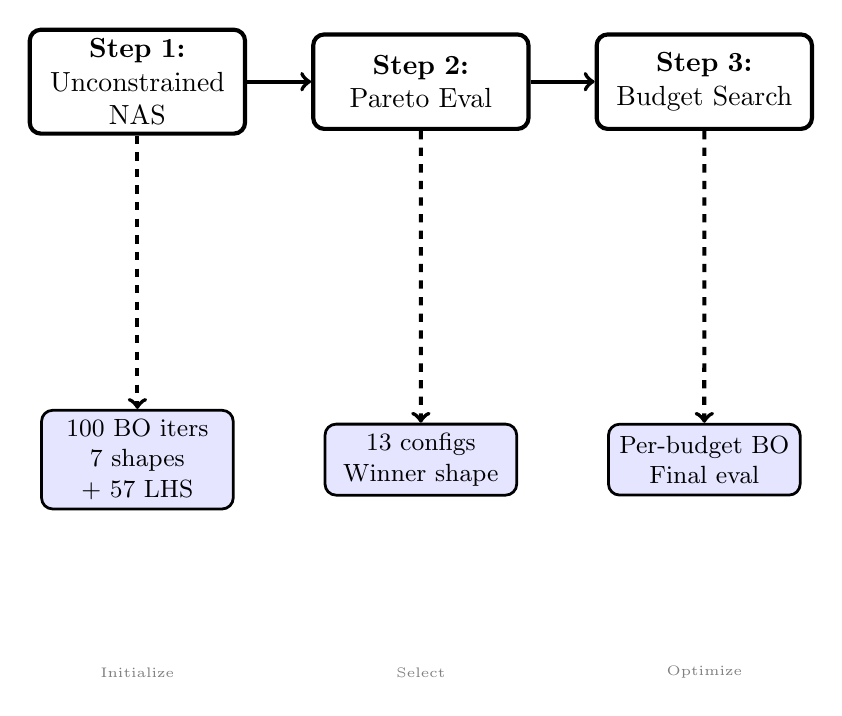
\begin{tikzpicture}[node distance=3cm, auto, scale=0.9]
  % Styles
  \tikzstyle{stage}=[rectangle, draw, fill=white, text width=2.5cm, text centered, rounded corners, minimum height=1.2cm, line width=1.5pt]
  \tikzstyle{output}=[rectangle, draw, fill=blue!10, text width=2.2cm, text centered, rounded corners, minimum height=0.9cm, font=\small, line width=1pt]
  \tikzstyle{arrow}=[->, thick, line width=1.5pt]

  % Stage 1
  \node[stage] (stage1) at (0, 0) {\textbf{Step 1:} \\ Unconstrained NAS};
  \node[output, below of=stage1, yshift=-1.8cm] (out1) {100 BO iters \\ 7 shapes + 57 LHS};

  % Stage 2
  \node[stage] (stage2) at (4, 0) {\textbf{Step 2:} \\ Pareto Eval};
  \node[output, below of=stage2, yshift=-1.8cm] (out2) {13 configs \\ Winner shape};

  % Stage 3
  \node[stage] (stage3) at (8, 0) {\textbf{Step 3:} \\ Budget Search};
  \node[output, below of=stage3, yshift=-1.8cm] (out3) {Per-budget BO \\ Final eval};

  % Arrows between stages
  \draw[arrow] (stage1) -- (stage2);
  \draw[arrow] (stage2) -- (stage3);

  % Vertical arrows to outputs
  \draw[arrow, dashed] (stage1) -- (out1);
  \draw[arrow, dashed] (stage2) -- (out2);
  \draw[arrow, dashed] (stage3) -- (out3);

  % Annotations
  \node[font=\tiny, gray, below of=out1, yshift=0.3cm] {Initialize};
  \node[font=\tiny, gray, below of=out2, yshift=0.3cm] {Select};
  \node[font=\tiny, gray, below of=out3, yshift=0.3cm] {Optimize};
\end{tikzpicture}